\chapter{基于transformer的气井产量预测算法及开关井推荐}
在气井的全生命周期任务中,气井产量预测可以帮助企业有效规划气井的开发和生产过程,确定最佳的生产速率,以避免资源浪费和确保气井的长期稳定产出。同时,
准确的产气量预测有助于企业评估气井的经济价值,从而做出更加明智的投资决策,比如决定是否继续开发新的气田或是对现有气井进行增产操作。在制定策略时,了解
未来的产气量可以帮助企业更有效地分配资源,比如人力、资金和设备,确保这些资源被投入到最有价值和最需要的地方。并有助于在有风险的情况下识别潜在的生产下
降风险和其他相关风险,使企业能够及时调整策略以降低损失。气井产气量预测是根据气井的生产动态历史数据,对气井未来一段时间内的产能做出准确评估。过去比较广泛
的进行产量预测的方法为预测气井的绝对无阻流量或者通过下降曲线分析的快速方法来匹配生产率-时间历史数据。但是这些现有的用于非常规储量估算的产量递减评估技术
具有潜在的局限性和一些特定假设,如对于间歇生产气井难以进行预测,这可能导致估计错误。本文采用时间序列预测的方式,目前油气产量时间序列预测的研究大多是同步
时间序列预测,应用场景有限。例如:不能实现使用井的静态参数及已知生产曲线预测未来生产曲线,也不能结合训练好的模型来优化生产设计。基于这些痛点,本章借鉴
了TFT的算法,同时根据企业的专家经验设计了网络模型,完成了气井产气量的时间序列预测任务。
\section{问题分析}
气井产量预测要求根据不同气井的历史产气量数据,构建预测模型;在推理阶段,模型能够对任一指定气井未来一段时间内的单日产气量做出预测。

在时间序列预测中,协变
量(covariates)是指与时间序列相关的其他变量。这些变量可以影响时间序列的行为和变化,因此在时间序列预测中使用协变量可以提高预测的准确性。协变量可以是任
何与时间序列相关的变量,包括经济指标、天气数据、人口统计数据等。例如,假设我们正在预测某个城市未来一周的销售额。此时,可以考虑将天气数据作为协变量,因为
天气可能会影响人们购买某些产品的决策。

气井产量预测任务可以抽象为一个多时间序列预测问题(约1000个时间序列),使用变量包括静态协变量(气井号,井丛号,集气站号,气井类别),随时间变化的协变量
(Time-dependent Inputs),可以细分为过去可知,未来不可知的协变量(Past-observed Inputs),如油压,套压,井口温度,以及过去和未来都可知的协变量
(Apriori-known Future Inputs),如气井已经生产的天数,每日开井时间。此处,每日开井时间是一个影响产气量的重要因素,因为若开井时间为0,则产气量必定
为0。未来时刻的开关井时间受人工调控开关井的影响,是可知的,因此可以设置为过去和未来都可知的协变量。
\section{问题描述}
\subsection{单井产气量预测问题描述}
对于单个气井,其输入是气井一段时间的产量数据及对应的气井动态数据。对于单井一段时间内的数据,将其记为
\begin{equation}
    \left\{ (x_{\delta}^i, x_{\rho}^i, x_{\sigma}^i, x_{\tau}^i, x_{h}^i, y^i_{\varphi }) \mid i = 1, 2, \ldots, T \right\}
    \label{eq:singlewell}
\end{equation}
其中\( T \)表示气井数据的总时间长度,其中上标$i$表示时刻$i$,下标表示不同的特征,分别如下所示:油压\( \delta \)、套压\( \rho \)、
井口温度\( \sigma \)、投产天数\( \tau \)、每日开井时间$h$、日产量$\varphi $。则问题可以定义为:基于气井过去一段时间内的油压\( \delta \)等数据来预测气井未来一段时间内的产量,记要预测的未来时间步长$t$。形式化
地描述其输入如公式\eqref{eq:sinpredic}所示。
\begin{equation}
    \left\{
    \begin{array}{ll}
    (x_{\tau}^i, x_{\rho}^i, x_{\sigma}^i, x_{\tau'}^i, x_{h}^i, y_{\varphi }^i) &  i = 1, 2, ..., T \\
    (x_{\tau}^{T+j}, x_{h}^{T+j}) & j = 1, 2, ..., t
    \end{array}
    \right.
    \label{eq:sinpredic}
\end{equation}    
输出为$\left\{ y^{T+1}_{\varphi}, y^{T+2}_{\varphi}, \ldots, y^{T+t}_{\varphi} \right\}$。

对于时序数据预测问题,需要将一整条数据依据时间点划分为训练数据和测试数据,然后需要设置训练数据步长与滑动步长,从而生成多个样本。因此为将问题转换为时间
序列问题,需设置新的符合并对问题作进一步地定义。需要将记训练数据输入步长为$T$,$T$通常大于等于要预测的时间步长$t$,记滑动步长为$s$,记训练数据和测试数
据的划分时间点为$N_0$,记$\mathbf{X_i} = \{x^i_\delta, x^i_\rho, x^i_\sigma, x^i_\tau, x^i_h\}, \quad \mathbf{Y_i} = y^i_\varphi$,则训练数据可以用式\eqref{eq:traindata}表示。
\begin{equation}
    \begin{aligned}
    x_{\text{train}}^{(1)} &: \{ (X_1, Y_1), ..., (X_{T}, Y_{T}), (x^{T+1}_{\tau }, x^{T+1}_{h }), ..., (x^{T+t}_{\tau }, x^{T+t}_{h}) \}, \\
    y_{\text{train}}^{(1)} &: \{Y_{T+1}, ... ,Y_{T+t}\}, \\
    x_{\text{train}}^{(2)} &: \{ (X_{1+s}, Y_{1+s}), ..., (X_{T+s}, Y_{T+s}), (x^{T+s+1}_\tau , x^{T+s+1}_h ), ..., (x^{T+s+t}_{\tau }, x^{T+s+t}_{h}) \}, \\
    y_{\text{train}}^{(2)} &: \{Y_{T+s+1}, ... ,Y_{T+s+t}\}, \\
    & \vdots
    \end{aligned}
    \label{eq:traindata}
\end{equation}
测试数据可以用式\eqref{eq:testdata}来表示。
\begin{equation}
    \begin{aligned}
    x_{\text{test}}^{(1)} &: \{ (X_{N_0}, Y_{N_0}), ..., (X_{N_0 + T}, Y_{N_0 + T}), (x^{N_0 + T+1}_{\tau }, x^{N_0 + T+1}_{h }), ..., (x^{N_0 + T+t}_{\tau }, x^{N_0 + T+t}_{h}) \}, \\
    y_{\text{test}}^{(1)} &: \{Y_{N_0 + T+1}, ... ,Y_{N_0 + T+t}\}, \\
    & \vdots
    \end{aligned}
    \label{eq:testdata}
\end{equation}
最终,问题定义为构建机器学习/深度学习预测器$f_{ML }$,根据一段连续生产的历史数据预测未来时间长度$t$内的流量,即
\begin{equation}
    (Y_{n+1}, \ldots, Y_{n+t}) = f_{ML}(X_n, Y_n, X_{n-1}, Y_{n-1}, \ldots, X_{n-T+1}, Y_{n-T+1}, X^{n+1}_{\tau}, X^{n+1}_{h}, X^{n+t}_{\tau}, X^{n+t}_{h})
\end{equation}
    
\subsection{多井产气量预测问题描述}
现有产气量预测方法多为针对某一单一气井的建模,应用价值有限。每个气井的产量主控因素可能有较大差别,且很多参数是无法量化的,无法加入到机器学习中,带来了
较大的不确定性。因此,通过某一单一气井时间序列数据训练出的机器学习模型往往无法针对其他气井使用。

同时,对于本企业提供的气井数据集而言,一共包含1000余口气井的时间序列数据。一方面,要针对单一气井构建不同的时间序列模型是不现实的,单井的数据量是有限的,且部分气井仅具
有极少量数据,无法据此构建机器学习/深度学习模型,且模型过多会导致通用性差,难以管理等问题。另一方面,使用所有气井的数据集进行训练可以捕捉到不同气井之
间具有的相似的生产规律,提高了模型泛化性,实现了对多气井产气量预测的统一建模。

本文的多气井产气量预测在单井产气量预测的基础上添加一系列静态协变量(包括气井号,井丛号,集气站号和气井类别),并针对第三章得到的不同类别的气井生成特定类别的预测结果。因此多气井产量预测模型在
考虑了气井预测模型的泛化性的基础上又不失特殊性,从而实现了气井产量的高效预测。

\section{数据处理及分类}
\label{sec:datafoc}
气井的数据在第\ref{cha:data}章已经选取了日期,集气站号,井序号,日产时间,井口压力(油压),套压,井口温度,日产量和投产时间等数据存储在了一
个名为GasProductionOri.csv的文件中。

但是此时的到的每条时间序列都过长,直接建模可能会由于计算资源的限制而变得不可行。为了统一输入输出格式,
降低模型复杂度和计算开销,本文使用滑动窗口技术将
训练数据切割为固定长度。滑动窗口模式是进行序列预测问题处理的最常用也是最有效方式,通过控制窗口的大小,可以调整参与预测的历史数据的数量。其模型如
图\ref{fig:slidewindow}所示。
\begin{figure}[H]
    \label{fig:slidewindow}
    \caption{滑动窗口数据分段示意图}
\end{figure}
如图\ref{fig:slidewindow}所示,设置滑动间隔为1,使用固定大小为4的滑动窗口,对气井的时间序列进行划分。在取出样本序列后,每个样本分段的数据差异大且复杂,
未经标准化处理的样本分段会导致机器学习模型的学习速度十分缓慢,甚至无法更新模型参数。同时,由于不同分段之间的差异,数值较大的分段可能会对模型的决策过程产生
不成比例的影响,导致模型偏向于这些数据,从而影响预测结果的准确性。我们需要对每个样本分段进行无量纲化处理,将所有特征放缩至$[0,1]$之间,即
\begin{equation}
    y = \frac{x - \text{min}}{\text{max} - \text{min}}
\end{equation}
其中$min$为该分段中的最小值,$max$为该分段中的最大值。

气井会因为它们的地理位置、地质构造、开采历史和技术等因素而表现出不同的产量特性。直接在所有气井数据上建立预测模型的话,模型就会过于复杂,难以捕捉到每一种类型气井的特点。而分类后,为每一类气
井建立模型可以简化问题,使得模型更容易泛化,减少过拟合的风险。同时,通过基于改进的K-Shape时间序列聚类算法对气井进行分类以后,可以将具
有相似产量特征的气井分为一组,使得预测模型能够专注于这些相似特征,从而提高预测准确性。第三章将气井分为 类,本章将分别对其进行产量预测。
\section{算法主要设计策略}
\subsection{算法框架}
根据上文所述内容,需要根据气井的历史数据信息来预测气井的未来产量。本文借鉴了TFT的框架,并根据企业的气井数据特征来对TFT的模型进行了一些改进。具体
的算法框架如图\ref{fig:TFTprogess}所示。
\begin{figure}[H]
    \label{fig:TFTprogess}
    \caption{基于transformer的气井产量预测算法流程图}
\end{figure}
本章提出的气井产量预测算法具体分为以下几个步骤:
(1)气井数据提取:本章使用企业提供的气井数据,并在第\ref{cha:data}章中对气井数据进行了数据清洗,使得其可以直接在接下来进行数据处理。

(2)气井数据预处理:使用滑动窗口对气井数据进行处理,接下来对数据进行无量纲化处理,将所有特征缩放至$[0,1]$之间。最终把得到数据集用于后续模型的训练、验证和测试。

(3)获取气井类别:根据第三章的方式对气井进行分类,以根据气井在地质特征、井深、压力水平和历史产量等不同条件下分类的结果分别进行预测。

(4)使用基于transformer的方式对每类气井分别进行预测:根据气井不同的协变量,将输入的历史时刻和未来时刻的特征经过一系列变换,得到一个抽象的
表征,然后分别输入到Encoder和Decoder中。Encoder部分使用GRU网络来编码历史时刻的信息,输出一个固定长度的向量,表示整个历史序列的含义。
Decoder部分使用自注意力机制来解码未来时刻的预测值,每个预测值都是根据之前所有时刻的加权结果得到的,这样可以提高模型的准确性。
如图\ref{fig:TFT}所示,为基于transformer的气井产量预测算法的模型结构图。
\begin{figure}
    \label{fig:TFT}
    \caption{基于transformer的气井产量预测算法的模型结构图}
\end{figure}
由图中可知,网络模型主要由门控残差网络、输入层、时间特征处理层、时域注意力层、position-wise前馈层以及分位数预测层组成。
\subsection{门控残差网络}
\label{cha:GRN}
由于输入与目标之间的关系是未知的,对于预测结果而言,到底需要什么程度的非线性处理是一项巨大的挑战。非线性层过多会出现梯度消失或梯度爆炸的问题,因此,有时
需要简化模型来处理问题。为了让模型只在需要的时候才灵活地应用非线性地方式处理数据,我们提出了门控残差网络来处理数据。门控残差网络的输入为主输入$\mathbf{a}$
和一个可选的上下文向量$\mathbf{c}$。具体操作如下所示:
\begin{equation}
    GRN_{\omega}(\mathbf{a}, \mathbf{c}) = \text{LayerNorm}(\mathbf{a} + GLU_{\omega}(\boldsymbol{\eta}_1))
\end{equation}
其中:
\begin{equation}
    \boldsymbol{\eta}_1 = \mathbf{W}_{1,\omega} \boldsymbol{\eta}_2 + \mathbf{b}_{1,\omega}
\end{equation}
\begin{equation}
    \boldsymbol{\eta}_2 = \text{ELU}(\mathbf{W}_{2,\omega} \mathbf{a} + \mathbf{W}_{3,\omega} \mathbf{c} + \mathbf{b}_{2,\omega})
    \label{eq:eta2}
\end{equation}
上式中,ELU是指线性激活函数,$\eta_1 \in \mathbb{R}^{d_{\text{model}}}$, $\eta_2 \in \mathbb{R}^{d_{\text{model}}}$ 是中间层,
LayerNorm是于2016年被提出的标准归一化,$\omega$ 是表示权重共享的索引。当$\mathbf{W}_{2,\omega} \mathbf{a} + \mathbf{W}_{3,\omega} \mathbf{c} + \mathbf{b}_{2,\omega} \gg 0$时,
ELU激活函数将作为恒等函数,而当$\mathbf{W}_{2,\omega} \mathbf{a} + \mathbf{W}_{3,\omega} \mathbf{c} + \mathbf{b}_{2,\omega} \ll 0$ 时,ELU激活函数产生一个固定的输出,直接触发线性层的行为。我们使用基于门控线性单元 (GLUs)的组件门控层来
提供灵活性,以抑制数据集中不需要的任何体系结构。假设 $\boldsymbol{\gamma } \in \mathbb{R}^{d_{\text{model}}}$ 是输入,GLU的形式为:
\begin{equation}
    GLU_{\omega}(\boldsymbol{\gamma }) = \sigma(\mathbf{W}_{4,\omega} \mathbf{\boldsymbol{\gamma }} + \mathbf{b}_{4,\omega}) \odot (\mathbf{W}_{5,\omega} \mathbf{\boldsymbol{\gamma }} + \mathbf{b}_{5,\omega}),
\end{equation}
其中 $\sigma(\cdot)$ 是sigmoid激活函数,$\mathbf{W}_{(\cdot)} \in \mathbb{R}^{d_{\text{model}} \times d_{\text{model}}}$ 是权重,$\mathbf{b}_{(\cdot)} \in \mathbb{R}^{d_{\text{model}}}$ 是偏置,
$\odot $ 是元素的Hadamard乘积。GLU允许模型控制GRN对原始输入$\mathbf{a}$的贡献程度--如果必要,GLU的输出可以都接近于0,以便抑制模型非线性
的贡献。对于没有上下文向量$\mathbf{c}$的实例,GRN简单地将上下文输入视为0(即在\eqref{eq:eta2}中,$\mathbf{c}=0$)。
\subsection{输入层}
本模型将融合了多种数据源。具体地由图中可知:输入层包括三种类型的变量。最左侧的$S$是静态变量,包括气井号、井丛号、集气站号和气井类别。从$x_{t-k}$到$x_t$代表的是从过去$k$时刻已知
,但未来不可知的随时间变化的变量,包括井口温度,油压,套压,日产量等。最右侧的$x_{t+1}$到$x_{t+\tau_{max}} $代表的是从过去$t-k$到未来$t+\tau_{max}$时刻
都可知的随时间变化的变量,包括已经投产的天数,每日开井时长等。

其中静态变量$S$需要经过静态协变量编码器来整合来自静态元数据的信息。具体地,本文使用\ref{cha:GRN}所展示的门控残差网络来编码产生上下文向量$\mathbf{c}_h$
,$\mathbf{c}_h$将传入时间特征的局部处理层作为GRU的初始输入。
\subsection{时间特征处理层}
在时间序列的数据中,重要的点例如异常、变化点或者周期性模式一般都是根据他们周围的值来识别的。通过编码时间序列能够在序列中记忆和使用先前的信息,增强局
部上下文,从而提高基于注意力架构模型的性能。本文将采用序列到序列层来进行时间序列编码,TFT使用LSTM来对时间序列进行编码,但是LSTM参数量相对较多,其包
括更多的门控单元。这会导致在训练和推理过程中需要更多的计算资源,特别是气井数据集的规模较大。尽管LSTM设计用来更好地捕捉长期依赖关系,但有时候它会
受到梯度消失或爆炸的影响,导致难以有效地学习长期依赖,这可能需要额外的技巧或者调整来解决。基于以上痛点,本文使用GRU来对时间序列进行编码。
GRU具有更简单的结构,它合并了LSTM的遗忘门和输入门,因此参数数量较少。这使得GRU在训练和推理过程中的计算效率更高。且其有更快的训练速度,。这使得在大规
模数据集上进行实验和调整参数时更加高效。我们将过去的输入序列$\bm{\xi}_{t-k:k}$提供给编码器,将未来的输入序列$\bm{\xi}_{t+1:t+\tau_{max}}$
提供给解码器。使用GRU生成一组均匀的时间特征,作为下一阶段的输入,用$\phi (t,n)$来表示,
其中$\phi(t,n) \in {\phi(t, -k), \ldots, \phi(t, T_{\text{max}})}$,$n$是位置指标。这种方式也可以完美处理观测到的过去和未来的输入不同而
存在的差异。同时,为了让静态数据也参与到时间序列变量的编码中,我们使用$\mathbf{c_h}$上下文向量初始化第一个GRU的隐藏状态。在此处也使用门控跳跃链接:
\begin{equation}
    \tilde{\bm{\phi}}(t, n) = \text{LayerNorm}\left(\tilde{\bm{\xi}}_{t+n} + \text{GLU}_{\tilde{\phi}}(\bm{\phi}(t, n))\right)
\end{equation}
其中$n \in [ -k, \tau_{\max}]$是位置指标。
\subsection{时域注意力层}
在进行GRU编码后,我们采用自注意力来学习不同时间步之间的长期关系。传统的多头注意力每个头使用不同的值,仅通过权重注意力本身并不能指示特定特征的重要性,此处
在传统多头注意力的基础上共享V。具体如下:
一般来说,注意力机制基于键矩阵\( K \in \mathbb{R}^{N \times d_{\text{attn}}} \)和查询矩阵\( Q \in \mathbb{R}^{N \times d_{\text{attn}}} \)
之间的关系对值\( V \in \mathbb{R}^{N \times d_v} \)进行缩放:
\begin{equation}
    \text{Attention}(Q, K, V) = A(Q,K)V
\end{equation}
其中$A()$是一个归一化函数,\( N \) 是进入注意力层的时间步数(即 \( k + t_{\text{max}} \))。常用的选择是缩放点积注意力:
\begin{equation}
    A(Q, K) = \text{Softmax}\left(\frac{QK^T}{\sqrt{d_{\text{attn}}}}\right)
\end{equation}
为了提高注意力机制的学习能力,Vaswani于2017年提出了多头注意力,使用不同的头针对不同的表示子空间:
\begin{equation}
    \text{MultiHead}(Q, K, V) = [H_1, \ldots, H_m]W_H
\end{equation}
\begin{equation}
    H_h = \text{Attention}(QW^Q_{(h)}, KW^K_{(h)}, VW^V_{(h)})
\end{equation}
其中\( W^K_{(h)} \in \mathbb{R}^{d_{\text{model}} \times d_{\text{attn}}} \), \( W^Q_{(h)} \in \mathbb{R}^{d_{\text{model}} \times d_{\text{attn}}} \), \( W^V_{(h)} \in \mathbb{R}^{d_{\text{model}} \times d_v} \) 
是针对键、查询和值的头特定权重 \( W_H \in \mathbb{R}^{m \cdot h \times d_{\text{model}}} \) 用于将所有头输出合并。
为了展示特定特征的重要性,做出的修改如下:
\begin{equation}
    \text{InterpretableMultiHead}(\mathbf{Q}, \mathbf{K}, \mathbf{V}) = \tilde{\mathbf{H}} \mathbf{W}_h
\end{equation}
\begin{equation}
    \begin{aligned}
        \mathbf{\tilde{H}} &= \tilde{A}(\mathbf{Q}, \mathbf{K}) \mathbf{V} \mathbf{W}_v, \\
        &= \left\{ \frac{1}{m_H} \sum_{h=1}^{m_H} A(\mathbf{Q} \mathbf{W}_Q^{(h)}, \mathbf{K} \mathbf{W}_K^{(h)}) \right\} \mathbf{V} \mathbf{W}_v, \\
        &= \frac{1}{m_H} \sum_{h=1}^{m_H} \text{Attention}(\mathbf{Q} \mathbf{W}_Q^{(h)}, \mathbf{K} \mathbf{W}_K^{(h)}, \mathbf{V} \mathbf{W}_v),
    \end{aligned}        
\end{equation}
式中:$\mathbf{W}_v \in \mathbb{R}^{d_{\text{model}} \times d_v}$是跨所有头共享的值的权重,$\mathbf{W}_h \in \mathbb{R}^{d_{\text{attn}} \times d_{\text{model}}}$
用于最终的线性映射。$\tilde{A}(\mathbf{Q}, \mathbf{K})$允许我们通过分析一组注意力权重来进行简单的可解释性研究。

在进行了时间特征处理层之后,我们应用注意力层。将所有的时间特征组合成单一的矩阵即$\bm{\varPhi }(t) = \left[ \bm{\phi} (t, -k), \ldots, \bm{\phi }(t, \tau_{\text{max}}) \right]^T$
并在每个时间点($N = \tau _{max} + k + 1$)应用时域注意力:
\begin{equation}
    \mathbf{B}(t) = \text{InterpretableMultiHead}(\mathbf{\varPhi }(t), \mathbf{\varPhi }(t), \mathbf{\varPhi }(t)),
\end{equation}
生成了$\mathbf{B}(t) = \left[ \mathbf{\beta }(t, -k), \ldots, \mathbf{\beta }(t, \tau_{\max}) \right]$。在自注意力层之后,增加了一个额外
的门控层来促进训练:
\begin{equation}
    \boldsymbol{\delta}(t, n) = \text{LayerNorm}(\boldsymbol{\phi }(t, n)) + \text{GLU}_{\boldsymbol{\delta}}(\boldsymbol{\beta}(t, n)).
\end{equation}
\subsection{position-wise前馈层}
对自注意力层应用额外的非线性处理,此处依然使用门控残差网络:
\begin{equation}
    \boldsymbol{\psi}(t, n) = \text{GRN}_{\boldsymbol{\psi}}(\boldsymbol{\delta}(t, n))
\end{equation}
其中$ \text{GRN}_{\boldsymbol{\psi}}$的权重在整个层中共享。此处还应用了一个跳过整个transformer块的残差连接,为序列到序列层提供了直接的路径。
倘若不需要额外的复杂性,就可以得到一个更简单的模型。如下所示:
\begin{equation}
    \tilde{\boldsymbol{\psi}}(t, n) = \text{LayerNorm}(\tilde{\boldsymbol{\phi}}(t, n)) + \text{GLU}_{\tilde{\boldsymbol{\psi}}}(\tilde{\boldsymbol{\psi}}(t, n))
\end{equation}
\subsection{分位数预测层}
借鉴了MQRNN框架的思路,本文采用分位数回归预测作为模型的输出方式。具体来说就是回归模型在对目标产量进行预测的时候不只预测$y$的一个期望值$\hat{y}$,
而是预测出$y$的概率分布中不同百分位数(如10\%,50\%,90\%)的值。分位数预测是根据上一步输出的线性变换生成的:
\begin{equation}
    \hat{\boldsymbol{y}}(q, t, \tau) = \mathbf{W}_q \tilde{\boldsymbol{\psi}}(t, \tau) + \mathbf{b}_q
\end{equation}
本文采用联合最小化分位数损失来训练模型,并将所有的分位数方法相加,具体如式\eqref{eq:loss}所示。
\begin{equation}
    \mathcal{L}(\Omega, \mathbf{W}) = \sum_{y_t \in \Omega} \sum_{q \in \mathcal{Q} } \sum_{\tau=1}^{\tau_{\max}} \frac{\text{QL}(y_t, \hat{\boldsymbol{y}}(q, t - \tau, t), q)}{M_{\tau_{\max}}}
    \label{eq:loss}
\end{equation}
其中$\text{QL}(y,\hat{y},q)$为分位数损失,具体定义如下:
\begin{equation}
    \text{QL}(y, \hat{y}, q) = q(y - \hat{y})_+ + (1 - q)(\hat{y} - y)_+,
\end{equation}
在式\eqref{eq:loss}中,$\Omega$是包含M个样本的训练数据,$W$表示模型的权重,$\mathcal{Q}$是分位数的集合(用户可自行指定,本文使用$\mathcal{Q} = \{0.4, 0.6\}$)。
\section{实验对比分析}
\subsection{数据集描述与环境说明}
基于transformer的气井产量预测算法会在第\ref{sec:datafoc}节提供的数据集上进行验证。本次实验的硬件环境为处理器Inter(R) Xeon(R) Silver 4261 cpu @ 2.10Hz,
显卡GeForce RTX 3090,内存256G,磁盘1T,操作系统采用Windows 10,开发环境为Pycharm,Python环境为Anaconda-4.12.0 python=3.9。
\subsection{评估指标}
为了验证本章所提出的基于transformer的气井产量预测算法的有效性,使用两个指标用于评估。其中一个是平均绝对误差(Mean Absolute Error, MAE),其可以衡量
预测值与实际值之间的平均绝对偏差。公式如式\eqref{eq:MAE}所示。
\begin{equation}
    MAE(y, y') = \frac{1}{n} \sum_{i=1}^{n} |y_i - y'_i|
    \label{eq:MAE}
\end{equation}
另一个常用误差指标为累计产量的相对误差,公式如式\eqref{eq:RCPE}所示。
\begin{equation}
    RCPE = \frac{\sum_{i=1}^{n} |y_i| - \sum_{i=1}^{n} |y'_i|}{\sum_{i=1}^{n} |y_i|}
    \label{eq:RCPE}
\end{equation}
上面两式中,$i$表示索引,用于遍历数据集中的每一个数据点。例如,如果我们有一个包含多个观测值的数据集,$i$就用来表示这些观测值的序号,从第一个观测值
到第$n$个观测值。$y$表示真实值,也就是实际产量,$\hat{y}$表示预测值,也就是通过模型预测得到的产量。
\subsection{LightGBM模型设计}
根据前文所述,本问题需要同时对1000余口气井构建时间序列预测模型,且问题包含多种类型的协变量,由第一章的国内外研究现状可知,机器学习模型中,当前对于时间序列预测问题的主流选择是特征工程+LightGBM模型的方法,这也是当前各大时间序列竞赛中大多数获胜方案所采用的策略。
下面将对LightGBM模型的设计做具体介绍。

决策树模型可以用于回归预测任务,其基本原理是将输入变量空间划分成多个子空间,并在每个子空间内拟合一个简单的回归模型。在预测时,将输入数据映射到对应的子空间,并用该子空间内的回归模型来进行预测,从而得到最终的预测结果。

集成树模型的原理是将多个弱学习器(例如决策树)组合成一个强学习器,从而提高预测的准确性和稳定性。在具体的实现中,集成树模型通常采用Bagging或Boosting的方法进行集成。其中Boosting是一种迭代式的方法,通过序列化训练多个决策树模型,每次训练的模型都会针对前一轮的错误进行优化,从而逐步提升模型的准确性。在Boosting中,还有一种著名的算法叫做梯度提升树(Gradient Boosting Tree),它通过在每轮迭代中拟合负梯度来进行模型训练。LightGBM(Light Gradient Boosting Machine)是一种基于决策树的梯度提升框架,是由微软亚洲研究院开发的。它具有高效性和准确性,尤其适用于处理大规模数据集。相较于其他梯度提升框架,LightGBM 在训练速度和内存使用方面具有优势。

多步时间序列预测是指根据历史数据来预测未来多个时刻的数据,例如预测未来一周的天气或销量。要使LightGBM模型适应于多步时间序列预测,需要进行以下几个步骤:

数据准备:对于本问题,需要将历史产气量数据按照气井号和时间顺序进行排序,并且将数据集划分为训练集,验证集和测试集。同时,需要对静态协变量和随时间变化的协变量进行特征工程处理。
数据准备过程分为数据清洗和数据划分,数据清洗如\ref{cha:data}所述,数据划分部分选取每口井最后一段forecast horizon长度的气井产量数据作为测试集(forecast horizon指要预测的长度,如对未来45天的每日产气量进行
预测),选取倒数第二个forecast horizon长度的气井产量数据作为验证集,验证集用来调整lightGBM模型的超参数,其余数据用作测试集。

对时间序列数据进行特征工程,抽取延迟特征、滑动窗口特征等。在该问题中,所选取的静态特征包括,集气站号Station,井丛号Cluster,气井号WellNo,配产量Allocation,其余特征包括表示时间的整数Elapsed,这个整数值通过当前日
期与数据集第一天的日期差计算得到,表示气井生产时长的整数值ElapsedProduction,通过当前日期与气井投产日期的日期差计算得到,当日开井时间DailyHour,延迟特征Lag1到Lag30,其中延迟特征Lagi表示当前日期前i天的产气量,即使
用过去的产气量数据预测未来产气量(这里以预测未来7天的产气量为例,使用过去30天的数据预测未来7天的产气量),滑动特征RollingMean7,RollingStd7,……,RollingMean180, RollingStd180,其中RollingMeani和RollingStdi分
别表示过去i天产气量数据的均值和方差,i取{7,15,30,60,180},通过Rolling特征提取历史产气量数据的数值信息。这里具体使用过去多长时间的历史数据对未来进行预测通常根据经验选取,通常这个长度在forecast horizon到2*forecast horizon之间。
进行特征工程后,构造训练数据,将每个时刻的产气量作为目标值和对应的特征作为一条样本。
\begin{figure}[H]
    \centering
    \caption{一条样本所包含的特征}
    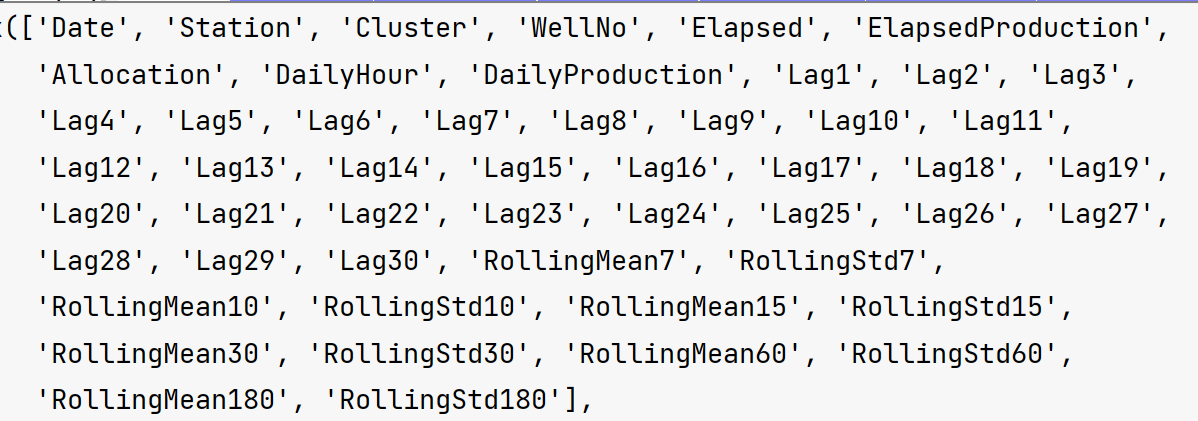
\includegraphics{figure/asamplefeature.png}
\end{figure}
如图\ref{fig:singlesample}表示一条训练样本(再加上进行特征工程Lag和Rolling特征),DailyProduction表示当日产气量,为目标值。
\begin{figure}[H]
    \centering
    \caption{单条样本示意图}
    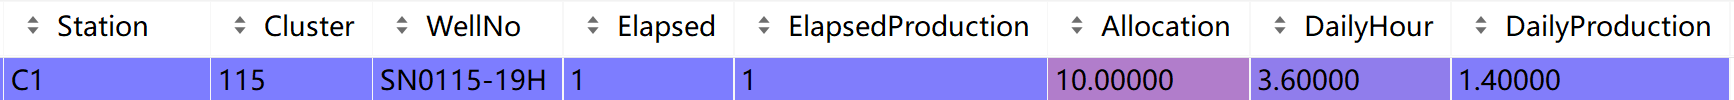
\includegraphics{figure/singlesample.png}
    \label{fig:singlesample}
\end{figure}
调整LightGBM模型的参数,根据不同
的目标函数、评价指标、学习率、树的深度、叶子节点数等进行手动或自动调优。最终模型选择超参数如图\ref{fig:LightGBMSuper}所示,使用huber损失函数,MAE作为指标来对模型预测效果拟合效果进行评价。
\begin{figure}[H]
    \centering
    \caption{LightGBM模型所选取的超参数}
    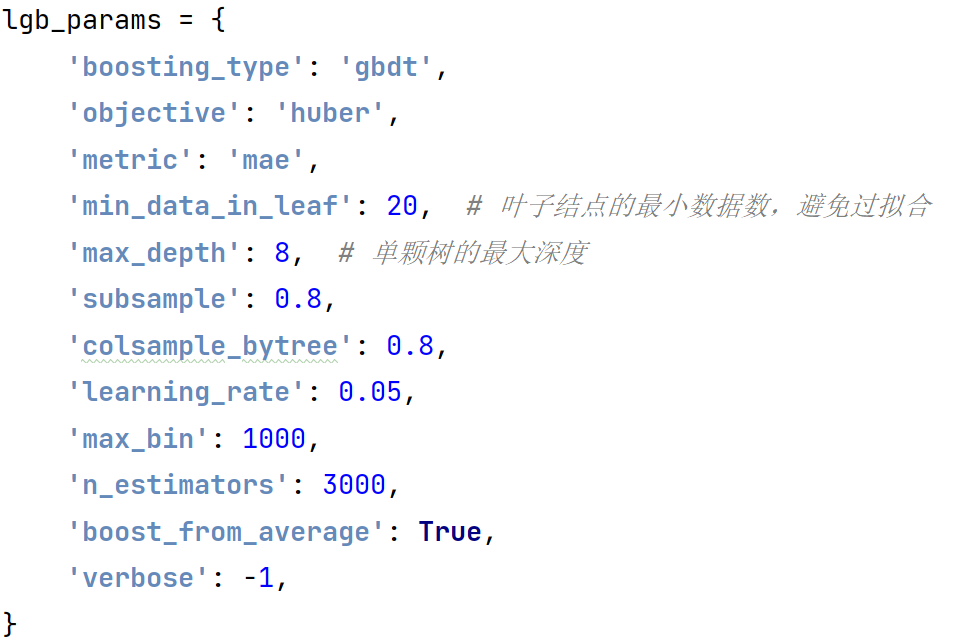
\includegraphics{figure/LightGBMsuper.png}
    \label{fig:LightGBMSuper}
\end{figure}
其中huber损失函数的定义如式\eqref{eq:huber}所示。
\begin{equation}
    L_{\delta}(y, f(x)) = 
        \begin{cases} 
        \frac{1}{2}(y - f(x))^2, & \text{if } |y - f(x)| \leq \delta \\
        \delta|y - f(x)| - \frac{1}{2}\delta^2, & \text{if } |y - f(x)| > \delta
        \end{cases}
    \label{eq:huber}
\end{equation}
在中,\(f(x)\)为预测值,δ为Huber损失函数的参数,δ接近0时,
Huber损失趋向于MAE。δ越大时,Huber损失趋向于MSE,在梯度下降时 MSE较MAE更为准确。而在异常值出现时 MAE较MSE更加鲁棒。Huber损失函数集中了两者的优势。这里MAE损失的定义为
\[MAE = |y - f(x)|,\]
MSE损失的定义为
\[MSE = (y - f(x))^2.\]

确定训练样本和模型超参数后,即可进行LightGBM模型的训练过程。在推理阶段,使用训练好的模型对于任一指定气井未来一段时间内的单日产气量做出预测。

在训练好的模型中,通过递归预测的方式,预测未来若干天的产气量。具体地,从当前时刻开始,先用模型预测未来第一天的产气量,然后将预测结果作为已知量(未来第二天地Lag1特征)输入到模型中,再预测未来第二天的产气量,以此类推。
\subsection{对比实验}
(1) 对比模型选择
根据前文所述,本问题需要同时对1000余口气井构建时间序列预测模型,且问题包含多种类型的协变量,因此初步选取基于注意力机制的seq2seq模型,lightGBM模型、TFT模型以及本文的模型这四个可以解决这类问题的模型进行实验。

经过对手头的单井日报数据进行处理,累计10年,1000余口气井约有总共约有160多万条数据。为了展示各算法的预测性能,选出3口井的产量数据作为测试集进行测试,分别是:SN0016-05, SN0004-04,SN0012-10。这3口井的近期
平均产量分别位于大于2,1到2之间,小于1区间(单位:$10^4m^3$).如表\ref{fig:modelselection}所示,基于注意力机制的seq2seq模型,由于模型结构限制,无法包含未来时刻的开关井信息,导致预测效果显著劣于其余三个模型。
lightGBM模型、TFT模型及本模型,预测准确率相近,本文算法略优于TFT和lightGBM模型,预测时间本文模型优于TFT和lightGBM模型。但是在模型训练阶段,lightGBM模型(10min)显著快于TFT模型(4h)及本文(2.5h)。故最终保留
本文中的模型和lightGBM模型。
\begin{table}[H]
    \renewcommand{\arraystretch}{1.5}
    \caption{模型选择实验结果}
    \label{fig:modelselection}
    \centering
    \begin{tabular}{|c|c|c|c|c|}
        \hline
        \textbf{测试对象} & \textbf{模型} & \textbf{MAE($10^4 \ m^3$)} & \textbf{RCPE(\%)} & \textbf{预测时间(s)} \\ \hline
        \multirow{4}{*}{SN0016-05}  & TFT          & 0.241                       & 3.14              & 8.369                \\ \cline{2-5}
                                    & LightGBM     & 0.262                       & 3.80              & 0.89                 \\ \cline{2-5}
                                    & Seq2seq      & 0.512                       & 10.25             & 5.25                 \\ \cline{2-5}
                                    & Ours         & 0.225                       & 3.02              & 7.29                 \\ \hline
        \multirow{4}{*}{SN0004-04}  & TFT          & 0.041                       & 1.39              & 12.9                 \\ \cline{2-5}
                                    & LightGBM     & 0.043                       & 1.40              & 0.92                 \\ \cline{2-5}
                                    & Seq2seq      & 0.132                       & 7.89              & 6.22                 \\ \cline{2-5}
                                    & Ours         & 0.036                       & 1.36              & 12.1                 \\ \hline
        \multirow{4}{*}{SN0012-10}  & TFT          & 0.103                       & 24.8              & 13.52                \\ \cline{2-5}
                                    & LightGBM     & 0.112                       & 27.0              & 1.03                 \\ \cline{2-5}
                                    & Seq2seq      & 0.153                       & 30.1              & 6.34                 \\ \cline{2-5}
                                    & Ours         & 0.095                       & 24.1              & 13.16                \\ \hline
    \end{tabular}
\end{table}
结合图中可以看出,本文的模型在MAE和RCPE指标上的表现均优于其他三种模型,TFT由于参数量太复杂训练和预测时间都较久,效果也稍次于本模型。相对而言,LightGBM模型预测时间较短且也可以取得相对较好的预测结果。
这表明在实时性要求较高的场景中,LightGBM模型可能是一个较好的选择。Seq2seq模型在这三个测试对象上的表现相对较差,可能需要进一步优化模型结构或参数。根据实验结果,可以得出结论:在这三个测试对象上,本模型的预测性能最佳,
但预测时间较长。当实时性要求较高时,可以考虑使用LightGBM模型。

(2)使用部分数据进行预测

本次实验的动机为:由于早期数据缺乏套压记录,这可能会影响预测模型的准确性。近期数据包含了所有重要特征,包括套压数据,并且能够代表整个时间序列的主要趋势和模式,那么只使用近期数据进行预测可能是一个合理的选择。
\begin{table}[h]
    \renewcommand{\arraystretch}{1.5}
    \centering
    \caption{使用部分数据集训练和使用全数据集训练的对比}
    \label{tab:alldatacomparison}
    \begin{tabular}{|c|c|c|c|c|}
    \hline
    \textbf{气井产量区间($10^4 \ m^3$)} & \multicolumn{2}{c|}{\textbf{MAE}} & \multicolumn{2}{c|}{\textbf{RCPE}} \\ 
    \cline{2-5} 
    \textbf{(}$10^4 m^3$\textbf{)} & 使用部分数据 & 使用全部数据 & 使用部分数据 & 使用全部数据 \\ 
    \hline
    大于4               & 0.267        & 0.367        & 0.022        & 0.051        \\ 
    \hline
    3至4               & 0.193        & 0.249        & 0.028        & 0.048        \\ 
    \hline
    2至3               & 0.136        & 0.130        & 0.042        & 0.042        \\ 
    \hline
    1至2               & 0.101        & 0.103        & 0.047        & 0.042        \\ 
    \hline
    小于1               & 0.120        & 0.122        & 0.165        & 0.163        \\ 
    \hline
    \end{tabular}
\end{table}
为对比预测效果,使用本文模型针对未来7天的产气量构建预测模型,分别使用所有数据和使用2017-01-01之后的数据构建两个不同的模型。根据近期平均产量将所有井划分为大于4,3到4之间,2到3之间,1到2之间,小于1这五类,每类类
别数分别为23,41,85,198,620.使用两种模型对这5类型的气井分别进行预测,要计算的预测准确性指标包括MAE(平均绝对误差)和RCPE(相对百分比误差)。对每类型井的预测指标进行统计,使用预测指标在每类型气井的中位数作为对
该类预测效果的近似表示。在测试过程中,存在部分井由于开井时间较晚,数据数小于时间序列预测的时间窗口,需对这部分井进行排除,此外,一些井在预测时间段内由于均处于关井状态,产气量为0,这部分井的预测缺乏统计学意义,同样予
以排除。
    
通过对每类型气井的预测指标进行统计,可以得出以下结论:

对于产量大于4的气井,使用2017-01-01之后的数据预测的MAE为0.267,而使用所有数据的MAE为0.367。同时,RCPE分别为0.022和0.051。这说明基于2017-01-01之后的数据构建的模型预测效果较好。对于产量在3到4之间的气井,使
用2017-01-01之后的数据预测的MAE为0.193,而使用所有数据的MAE为0.249。同时,RCPE分别为0.028和0.048。这同样说明基于2017-01-01之后的数据构建的模型预测效果较好。对于产量在2到3之间的气井,MAE和RCPE分别
为0.136、0.130和0.042、0.042。在这个区间,两个模型的预测效果相当。对于产量在1到2之间的气井,使用2017-01-01之后的数据预测的MAE为0.101,而使用所有数据的MAE为0.103。同时,RCPE分别为0.047和0.042。在这个区间,两个
模型的预测效果相当,但基于2017-01-01之后的数据构建的模型在MAE上略好。对于产量小于1的气井,使用2017-01-01之后的数据预测的MAE为0.120,而使用所有数据的MAE为0.122。同时,RCPE分别为0.165和0.163。在这个区间,两个模
型的预测效果相当,但基于所有数据构建的模型在RCPE上略好。

综上所述,在大部分产量区间中,基于2017-01-01之后的数据构建的模型预测效果都较好,但在产量较低的区间中,两个模型的预测效果相当。

(3)本模型和LightGBM模型对比

实验基本设置: 在这个实验中,我们选用本模型和LightGBM(一种基于梯度提升决策树的机器学习模型)对未来7天的产气量进行预测。实验结果是对属于该日均产气量范围内的所有气井进行预测并计算其指标的中位数统计值得到的。
\begin{table}[H]
    \renewcommand{\arraystretch}{1.5}
    \centering
    \caption{本文模型和LightGBM模型预测结果对比}
    \label{tab:prediction_comparison}
    \begin{tabular}{|c|c|c|c|}
    \hline
    模型     & 预测时间区间 & MAE($10^4 m^3$) & RCPE(\%) \\ \hline
    LightGBM & 小于 1      & 0.128           & 0.228    \\ \hline
    LightGBM & 1 到 2      & 0.136           & 0.093    \\ \hline
    LightGBM & 大于 2      & 0.149           & 0.043    \\ \hline
    Ours      & 小于 1      & 0.122           & 0.163    \\ \hline
    Ours      & 1 到 2      & 0.102           & 0.047    \\ \hline
    Ours      & 大于 2      & 0.163           & 0.035    \\ \hline
    \end{tabular}
\end{table}
实验结果对比与分析: 根据上述统计结果表格,可以看出:

对于日均产气量小于1的气井,本文模型的MAE和RCPE分别为0.122和0.163,而LightGBM模型分别为0.128和0.228。在这种情况下,本文模型的预测性能更好。

对于日均产气量在1到2之间的气井,本文模型的MAE和RCPE分别为0.102和0.047,而LightGBM模型分别为0.136和0.093。在这种情况下,本文模型的预测性能也更好。

对于日均产气量大于2的气井,本文模型的MAE和RCPE分别为0.163和0.035,而LightGBM模型分别为0.149和0.043。在这种情况下,尽管本文模型在RCPE上的表现更好,但在MAE上,LightGBM模型的表现更优。

实验中对于日产量大于2的气井,选取123口井的测试结果作为有效数据,对于日产气量在1到2之间的气井,选取184口井的测试结果作为有效数据,对于日产气量小于1的气井,选取459口井的测试结果作为有效数据。

从预测性能上看,本文模型在各种情况下都表现出较好的预测性能。然而,从实用性的角度来看,LightGBM模型的训练和预测时间要远远低于本文模型。具体来说,LightGBM模型的重训练时间为5分钟,而本文模型为1.5小时;LightGBM模型
的预测时间平均约为1.2秒,而本文模型平均约为7.5秒。这意味着,在实际应用中,使用LightGBM模型会更加节省时间和计算资源。

总结:从实验结果来看,本文模型在预测性能上具有优势,但在实用性方面,LightGBM模型具有更好的表现。因此,在实际应用中,需要根据实际需求的精度和计算资源进行权衡,选择合适的模型。
\subsection{实验结果统计值展示}
为完整展示实验结果,分别列出两种预测模型分别在预测步长为7天和45天时的预测结果统计指标,统计指标不仅包括中位数,还包括平均数,\%25分位数,75\%分位数,标准差。
产量区间小于1、1到2、大于2三种类型测试气井数量分别为123、184、459。预测步长7天的MAE结果如表\ref{tab:MAE7}所示。
\begin{table}[H]
    \renewcommand{\arraystretch}{1.5}
    \centering
    \caption{本文模型和LightGBM模型预测未来7天内产气量预测结果的MAE指标对比}
    \label{tab:MAE7}
    \begin{tabular}{|c|c|c|c|c|c|c|}
    \hline
    模型     & 预测时间区间 & MAE mean & MAE std & MAE 25\% & MAE 50\% & MAE 75\% \\ \hline
    LightGBM & 小于 1      & 0.199    & 0.221   & 0.055    & 0.128    & 0.277    \\ \hline
    LightGBM & 1 到 2      & 0.180    & 0.179   & 0.069    & 0.136    & 0.211    \\ \hline
    LightGBM & 大于 2      & 0.249    & 0.286   & 0.087    & 0.149    & 0.297    \\ \hline
    Ours      & 小于 1      & 0.174    & 0.274   & 0.067    & 0.122    & 0.205    \\ \hline
    Ours      & 1 到 2      & 0.170    & 0.220   & 0.061    & 0.102    & 0.186    \\ \hline
    Ours      & 大于 2      & 0.300    & 0.454   & 0.089    & 0.163    & 0.298    \\ \hline
    \end{tabular}
\end{table}
预测步长7天的RCPE结果如表\ref{tab:RCPE7}所示。
\begin{table}[H]
    \renewcommand{\arraystretch}{1.5}
    \centering
    \caption{本文模型和LightGBM模型预测未来7天内产气量预测结果的RCPE指标对比}
    \label{tab:RCPE7}
    \begin{tabular}{|c|c|c|c|c|c|c|} % Change 'l' to 'c' for center alignment
    \hline
    模型     & 预测时间区间 & RCPE mean & RCPE std & RCPE 25\% & RCPE 50\% & RCPE 75\% \\ \hline
    LightGBM & 小于 1      & 0.433     & 0.845    & 0.097     & 0.228     & 0.477     \\ \hline
    LightGBM & 1 到 2      & 0.131     & 0.147    & 0.038     & 0.093     & 0.167     \\ \hline
    LightGBM & 大于 2      & 0.085     & 0.125    & 0.020     & 0.043     & 0.094     \\ \hline
    Ours      & 小于 1      & 0.363     & 0.757    & 0.066     & 0.163     & 0.358     \\ \hline
    Ours      & 1 到 2      & 0.112     & 0.187    & 0.016     & 0.047     & 0.098     \\ \hline
    Ours      & 大于 2      & 0.086     & 0.147    & 0.015     & 0.035     & 0.080     \\ \hline
    \end{tabular}
\end{table}
预测步长45天的MAE结果如表\ref{tab:MAE45}所示。
\begin{table}[H]
    \renewcommand{\arraystretch}{1.5}
    \centering
    \caption{本文模型和LightGBM模型预测未来45天内产气量预测结果的MAE指标对比}
    \label{tab:MAE45}
    \begin{tabular}{|c|c|c|c|c|c|c|}
    \hline
    模型       & 预测时间区间 & MAE mean & MAE std & MAE 25\% & MAE 50\% & MAE 75\% \\ \hline
    LightGBM  & 小于 1      & 0.198    & 0.151   & 0.091    & 0.159    & 0.273    \\ \hline
    LightGBM  & 1 到 2      & 0.245    & 0.191   & 0.106    & 0.186    & 0.306    \\ \hline
    LightGBM  & 大于 2      & 0.360    & 0.329   & 0.151    & 0.253    & 0.418    \\ \hline
    Ours       & 小于 1      & 0.132    & 0.113   & 0.058    & 0.110    & 0.181    \\ \hline
    Ours       & 1 到 2      & 0.217    & 0.207   & 0.077    & 0.130    & 0.272    \\ \hline
    Ours       & 大于 2      & 0.346    & 0.319   & 0.111    & 0.245    & 0.459    \\ \hline
    \end{tabular}
\end{table}
预测步长45天的RCPE结果如表\ref{tab:RCPE45}所示。 
\begin{table}[H]
    \renewcommand{\arraystretch}{1.5}
    \centering
    \caption{本文模型和LightGBM模型预测未来45天内产气量预测结果的RCPE指标对比}
    \label{tab:RCPE45}
    \begin{tabular}{|c|c|c|c|c|c|c|}
    \hline
    模型       & 预测时间区间 & RCPE mean & RCPE std & RCPE 25\% & RCPE 50\% & RCPE 75\% \\ \hline
    LightGBM  & 小于 1      & 0.384     & 0.750    & 0.089     & 0.201     & 0.396     \\ \hline
    LightGBM  & 1 到 2      & 0.117     & 0.121    & 0.029     & 0.074     & 0.160     \\ \hline
    LightGBM  & 大于 2      & 0.091     & 0.107    & 0.028     & 0.056     & 0.114     \\ \hline
    Ours       & 小于 1      & 0.361     & 1.731    & 0.071     & 0.146     & 0.319     \\ \hline
    Ours       & 1 到 2      & 0.112     & 0.128    & 0.026     & 0.072     & 0.146     \\ \hline
    Ours       & 大于 2      & 0.087     & 0.094    & 0.019     & 0.047     & 0.120     \\ \hline
    \end{tabular}
\end{table}
为直观展示预测结果,随机选择5口气井的预测结果如下文所示。
\section{开关井推荐}
本小节将介绍开关井策略推荐实际问题的解决办法。首先收集数据,包括井口产气量、井底压力、温度、环境温度、气价、能源成本等相关参数。同时也需
要采集各个气井的位置和特征等信息,以便进行搜索和选择。其次,根据实际情况和目标函数,选择合适的搜索算法。常见的搜索算法包括深度优先搜索、蚁群算法等。
不同算法有不同的优缺点,需要根据实际情况进行评估和选择。然后确定搜索空间,搜索空间即可选取的所有井的集合,需要考虑到可行性和搜索效率的平衡。通常可
以根据实际条件和目标函数,设置一些限制条件来缩小搜索空间,以提高搜索效率。接下来要执行搜索算法,根据设定的搜索算法,对搜索空间进行搜索。在搜索过程
中,需要按照目标函数的要求,评估不同井进行开关的效果,并记录每次开关井的结果和成本。在搜索完成后,需要对所有开关井的结果进行评估,选取最优的开关井方案。
评估时需要考虑到产量、成本、环境、管网模型等多方面因素,并综合权衡不同因素的影响,以选取最优的开关井方案。最后根据最优的开关井方案,实施相应的开关井策略。

气井开采过程中,通常会产生一定量的液体,包括水和油。产液量的增加会影响气井的产气量,因为液体在井筒中的积累会增加井筒的阻力,使气流的速度降低,
从而影响气井的产气量。当气井处于低压低产阶段时,气相不能有效地携带液体,会导致积液现象。此时,如采用间歇生产方式(即周期性地开关井),可以利用
关闭期间积累的压力差,在开启时将积聚在底部或中部的液体迅速排出。
但如果开关频率过高或关闭时间过短,则可能造成反复积排液、增加摩阻损失、降低生产效率。可若是开关频率过低或关闭时间过长,则可能导致底部水锥突
破、增加水含率、降低天然气质量。
\subsection{数据}
本小节使用过去三十天的井口温度、压力、开关井时间、产气量值并借助前文训练的产气量模型来预测未来七天内每口井的预计产气量;本文使用前一天的井口温度、压力以
及井丛的拓扑关系图等数据构建管网模型,计算压力差;通过对过去一段时间历史数据的总结得到每口井的开关井周期。
\subsection{管网模型}
在处理复杂的地下流体动力学问题时,精确的解析解往往难以获得。在某些情况下,特别是考虑到地层的渗透性、流体的粘度以及井筒和储层之间的压力交互作用时,压力沿
井深的变化近似于二次曲线。此处在计算平均压力时根据此理论采用了一个简化的假设,即压力分布沿井深呈二次曲线分布。在这个假设下,可以通过连接干管井丛的井口压
力平均值(P1)和管道出口压力,即集气站进站压力(P2)计算出平均压力(avgPressure)。具体公式如式\eqref{eq:avgPressure}所示。
\begin{equation}
    \text{avgPressure} = \frac{2.0 \times (P1^3 - P2^3)}{3.0 \times (P1^2 - P2^2)}
    \label{eq:avgPressure}
\end{equation}
式中,P1 和 P2 分别代表两个不同深度的压力值。

本文使用了一种经验模型来计算临界温度(Tpc)和临界压力(Ppc)。这个模型是基于大量实验数据得出的,它将气体相对密度($\delta$ )作为输入参数。
\begin{equation}
    T_{pc} = 93.3 + 181 \times \delta - 7 \times \delta^2
\end{equation}
\begin{equation}
    P_{pc} = 4.668 + 0.103 \times \delta - 0.259 \times \delta^2
\end{equation}
式中的气体相对密度$\delta$的默认取值为0.5962(无量纲)。

将实际温度(K)和平均压力(avgPressure)分别除以临界温度(Tpc)和临界压力(Ppc),得到温度和压力的缩减值(即相对于临界温度和临界压力的温度和压力)Tr和Pr。
\begin{equation}
    T_r = \frac{K}{T_{pc}}
\end{equation}
\begin{equation}
    P_r = \frac{\text{avgPressure}}{P_{pc}}
\end{equation}
式中K为开尔文温度$K = C + 273.15$。

压缩因子(Z-factor)是一个描述气体实际体积与理论(理想气体状态下的)体积之比的参数,是用于石油和天然气工程中评估气体的压缩性质的重要工具。压缩因子的值表明了实际气体与理想气体状态方程之间的偏离程度。

赞达尔方程\cite{Dranchuk1975CalculationOZ}(也称为Dranchuk-Aboukassem方程),是一种基于实验数据得出的经验公式,用于计算特定条件下的气体压缩因子。这个方程考虑了温度和压力的缩减值。具体公式如式\eqref{eq:Z-factor}所示。
\begin{equation}
    Z = 1 - \frac{3.52 \times P_r}{10^{0.9813T_r}} + \frac{0.274 \times P_r \times P_r}{10^{0.8157T_r}}
    \label{eq:Z-factor}
\end{equation}
通过使用该方程,可以在已知缩减温度和缩减压力的情况下,估计出天然气在特定温度和压力条件下的压缩因子,进而帮助工程师们更准确地预测和计算气体的行为和性能。
本式对于理解和计算实际天然气在地下储藏和输送过程中的物理行为至关重要。它使工程师能够更好地设计和优化天然气的提取、处理和运输系统。

最后,可以使用Darcy-Weisbach方程\cite{brown2002history}来计算压力。这个方程描述了气体在管道中流动时,由于摩擦损失而引起的压力降。在这里,需要考虑到气体的压缩性,因此使用压缩因子(Z)来修正方程。
\begin{equation}
    \text{calP1} = \left(P2^2 + 3.948 \times 10^{-8} \times Q \times Q \times \delta \times K \times \frac{L}{d^{1.6}}\right)^{0.5}
\end{equation}
此处Q代表产气量,单位为万方/日,在计算中需要进行单位换算。d是气井的管径,单位为毫米,默认取值为20。
当应用场景为气井传输管道(从井丛传输至集气站)时,$calP1$和$P1 - calP1$具有以下实际意义。

$calP1$:这个值表示计算得到的管道起点(如单口气井)的压力。它反映了在给定的生产条件(温度、产气量等)以及管道参数(长度、直径等)下,为了克服管道摩擦损失所需要的起始压力。 

$P1 - calP1$:这个值表示实际管道起点压力(P1)与计算得到的起点压力($calP1$)之间的差值。这个差值可以用来评估管道的性能和系统效率。以下是几种可能的情况:

当$P1 - calP1$接近于零时,表示实际压力和计算压力非常接近,说明管道系统运行良好,摩擦损失在可接受范围内。 

当$P1 - calP1$为正值时,表示实际起点压力高于计算压力。这可能意味着管道系统存在过高的摩擦损失或是管道中存在堵塞等异常现象。 

当$P1 - calP1$为负值时,表示实际起点压力低于计算压力。这可能意味着管道系统效率较高,但也可能导致管道中的气体流量不足,从而影响到集气站的运行。 

通过分析$calP1$和$P1 - calP1$这两个值,可以为气井生产提供有用信息,有助于对生产参数进行调整和优化,提高气井生产效率和安全性。同时,这些信息也可以用于诊断管道系统是否存在异常,以便及时采取纠正措施。
\subsection{搜索算法}
基于对实际问题的分析,借助FOA算法来完成搜索。
主要对FOA算法中的距离进行了自定义:

当目前产量$current\_amount>target$(预计想要达到的总产量),系统需要从开着的井中选择一口井关闭,这时认为距离函数与压力差$delta\_pressure$和已经开井时间$open\_time$高度相关,因此距离函数定义如\eqref{eq:closewell}所示。
\begin{equation}
    \text{Dist}_i = \frac{1}{\sqrt{{\text{delta\_pressure}_i}^2 + {\text{open\_time}_i}^2}}
    \label{eq:closewell}
\end{equation}
当目前产量$current\_amount<target$时,系统需要从可以开的井中选择一口井打开,本文认为压力差越小越好,产气量越大越好,因此距离函数与产气量、压力差有关,距离函数的定义如如\eqref{eq:openwell}
\begin{equation}
    \text{Dist}_i = \frac{\sqrt{{\text{delta\_pressure}_i}^2}}{\sqrt{{\text{pre\_production}_i}^2}}
    \label{eq:openwell}
\end{equation}
将当前问题代入到果蝇优化算法具体的步骤如\ref{al:openwell}所示。
\begin{algorithm}[H]
    \caption{基于果蝇优化的开关井推荐算法}
    \begin{algorithmic}[1]
       \Require 目标产气量target区间,前一天的开关井情况
       \Ensure  新的开关井策略
       \State 初始化,以第一天的开关井情况作为初始值 init()
       \While{true}
            \If{current\_amount $>$ target}
                \State 随机分配方向、距离,搜索出一定数量可以关的井 update()
            \ElsIf{current\_amount $<$ target}
                \State 随机分配方向、距离,搜索出一定数量可以开的井 update()
            \Else
                \State \Return 最终开关井策略
            \EndIf
            \State 计算自定义的种群适应度
            \State 果蝇位置更新
        \EndWhile
    \end{algorithmic}
    \label{al:openwell}
\end{algorithm}
\subsection{搜索空间}
在实际生产过程中,不是所有的关着井都可以开,需要动态的挑出这些可以开的井。根据分析,本文排除下面这些井,在这个周期不投入生产。

1.去除用户前端自定义输入的尚不参与生产的井;

2.根据历史数据计算开关井周期,如果某口井当前已经开井时间大于最大开井时间,则排除这口井;

3.基于管网模型计算压力差,并根据用户输入阈值去除压力差过大的井;

4.单口井的生产能力太低的井。
\subsection{开关井推荐实验结果}
